%%% The main file. It contains definitions of basic parameters and includes all other parts.

%% Settings for single-side (simplex) printing
% Margins: left 40mm, right 25mm, top and bottom 25mm
% (but beware, LaTeX adds 1in implicitly)
\documentclass[12pt,a4paper]{report}
\setlength\textwidth{145mm}
\setlength\textheight{247mm}
\setlength\oddsidemargin{15mm}
\setlength\evensidemargin{15mm}
\setlength\topmargin{0mm}
\setlength\headsep{0mm}
\setlength\headheight{0mm}
% \openright makes the following text appear on a right-hand page
\let\openright=\clearpage

%% Settings for two-sided (duplex) printing
% \documentclass[12pt,a4paper,twoside,openright]{report}
% \setlength\textwidth{145mm}
% \setlength\textheight{247mm}
% \setlength\oddsidemargin{14.2mm}
% \setlength\evensidemargin{0mm}
% \setlength\topmargin{0mm}
% \setlength\headsep{0mm}
% \setlength\headheight{0mm}
% \let\openright=\cleardoublepage

\usepackage[usenames]{xcolor}  % typesetting in color

%% Generate PDF/A-2u
\usepackage[a-2u]{pdfx}

%% Character encoding: usually latin2, cp1250 or utf8:
\usepackage[utf8]{inputenc}

%% Prefer Latin Modern fonts
\usepackage{lmodern}

%% Further useful packages (included in most LaTeX distributions)
\usepackage{amsmath}        % extensions for typesetting of math
\usepackage{amsfonts}       % math fonts
\usepackage{amsthm}         % theorems, definitions, etc.
\usepackage{bbding}         % various symbols (squares, asterisks, scissors, ...)
\usepackage{bm}             % boldface symbols (\bm)
\usepackage{graphicx}       % embedding of pictures
\usepackage{fancyvrb}       % improved verbatim environment
\usepackage{natbib}         % citation style AUTHOR (YEAR), or AUTHOR [NUMBER]
\usepackage[nottoc]{tocbibind} % makes sure that bibliography and the lists
			    % of figures/tables are included in the table
			    % of contents
\usepackage{dcolumn}        % improved alignment of table columns
\usepackage{booktabs}       % improved horizontal lines in tables
\usepackage{paralist}       % improved enumerate and itemize

%% SPECIMEN
% Parts marked as SPECIMEN are used for building the example PDF.
% When the official template is generated by ./mkdist, all such parts
% are deleted, as well as all calls of \X and \XXX macros.
\def\X#1{\textcolor{red}{[#1]}}
\def\XXX#1{\par\smallskip\noindent \textcolor{red}{[#1]}}
%% NEMICEPS

%%% Basic information on the thesis

% Thesis title in English (exactly as in the formal assignment)
\def\ThesisTitle{Thesis title \X{as in the formal assignment}}

% Author of the thesis
\def\ThesisAuthor{Name Surname}

% Year when the thesis is submitted
\def\YearSubmitted{YEAR}

% Name of the department or institute, where the work was officially assigned
% (according to the Organizational Structure of MFF UK in English,
% or a full name of a department outside MFF)
\def\Department{Name of the department \X{as per Organizational Structure of MFF UK in English}}

% Is it a department (katedra), or an institute (ústav)?
\def\DeptType{Department}

% Thesis supervisor: name, surname and titles
\def\Supervisor{Supervisor's Name \X{+titles}}

% Supervisor's department (again according to Organizational structure of MFF)
\def\SupervisorsDepartment{department}

% Study programme and specialization
\def\StudyProgramme{study programme}
\def\StudyBranch{study branch}

% An optional dedication: you can thank whomever you wish (your supervisor,
% consultant, a person who lent the software, etc.)
\def\Dedication{%
Dedication.
}

% Abstract (recommended length around 80-200 words; this is not a copy of your thesis assignment!)
\def\Abstract{%
Abstract. \X{Recommended length around 80--200 words. This is not a~copy of your thesis assignment!}
}

% 3 to 5 keywords (recommended), each enclosed in curly braces
\def\Keywords{%
{key} {words} \X{usually 3 to~5 key words or phrases}
}

%% The hyperref package for clickable links in PDF and also for storing
%% metadata to PDF (including the table of contents).
%% Most settings are pre-set by the pdfx package.
\hypersetup{unicode}
\hypersetup{breaklinks=true}

% Definitions of macros (see description inside)
%%% This file contains definitions of various useful macros and environments %%%
%%% Please add more macros here instead of cluttering other files with them. %%%

%%% Minor tweaks of style

% These macros employ a little dirty trick to convince LaTeX to typeset
% chapter headings sanely, without lots of empty space above them.
% Feel free to ignore.
\makeatletter
\def\@makechapterhead#1{
  {\parindent \z@ \raggedright \normalfont
   \Huge\bfseries \thechapter. #1
   \par\nobreak
   \vskip 20\p@
}}
\def\@makeschapterhead#1{
  {\parindent \z@ \raggedright \normalfont
   \Huge\bfseries #1
   \par\nobreak
   \vskip 20\p@
}}
\makeatother

% This macro defines a chapter, which is not numbered, but is included
% in the table of contents.
\def\chapwithtoc#1{
\chapter*{#1}
\addcontentsline{toc}{chapter}{#1}
}

% Draw black "slugs" whenever a line overflows, so that we can spot it easily.
\overfullrule=1mm

%%% Macros for definitions, theorems, claims, examples, ... (requires amsthm package)

\theoremstyle{plain}
\newtheorem{thm}{Theorem}
\newtheorem{lemma}[thm]{Lemma}
\newtheorem{claim}[thm]{Claim}

\theoremstyle{plain}
\newtheorem{defn}{Definition}

\theoremstyle{remark}
\newtheorem*{cor}{Corollary}
\newtheorem*{rem}{Remark}
\newtheorem*{example}{Example}

%%% An environment for proofs

%%% FIXME %%% \newenvironment{proof}{
%%% FIXME %%%   \par\medskip\noindent
%%% FIXME %%%   \textit{Proof}.
%%% FIXME %%% }{
%%% FIXME %%% \newline
%%% FIXME %%% \rightline{$\square$}  % or \SquareCastShadowBottomRight from bbding package
%%% FIXME %%% }

%%% An environment for typesetting of program code and input/output
%%% of programs. (Requires the fancyvrb package -- fancy verbatim.)

\DefineVerbatimEnvironment{code}{Verbatim}{fontsize=\small, frame=single}

%%% The field of all real and natural numbers
\newcommand{\R}{\mathbb{R}}
\newcommand{\N}{\mathbb{N}}

%%% Useful operators for statistics and probability
\DeclareMathOperator{\pr}{\textsf{P}}
\DeclareMathOperator{\E}{\textsf{E}\,}
\DeclareMathOperator{\var}{\textrm{var}}
\DeclareMathOperator{\sd}{\textrm{sd}}

%%% Transposition of a vector/matrix
\newcommand{\T}[1]{#1^\top}

%%% Various math goodies
\newcommand{\goto}{\rightarrow}
\newcommand{\gotop}{\stackrel{P}{\longrightarrow}}
\newcommand{\maon}[1]{o(n^{#1})}
\newcommand{\abs}[1]{\left|{#1}\right|}
\newcommand{\dint}{\int_0^\tau\!\!\int_0^\tau}
\newcommand{\isqr}[1]{\frac{1}{\sqrt{#1}}}

%%% Various table goodies
\newcommand{\pulrad}[1]{\raisebox{1.5ex}[0pt]{#1}}
\newcommand{\mc}[1]{\multicolumn{1}{c}{#1}}


%%% MY MACROS
\newcommand{\todoA}[1]{[TODO A: #1]}  % urcite nutno
\newcommand{\todoB}[1]{[TODO B: #1]}  % bylo skoda to tam nedat
\newcommand{\todoC}[1]{[TODO C: #1]}  % pridal bych kdybych mel cas

\newcommand{\jh}[1]{[JH: #1]}  % komentar Jiriho Hany


% Title page and various mandatory informational pages
\begin{document}
%%% Title page of the thesis and other mandatory pages

%%% SPECIMEN
%%% Inscriptions at the opening page of the hard cover
\todoA{remove}

\pagestyle{empty}
\hypersetup{pageanchor=false}
%\XXX{Opening page of the hard cover. Not a part of the electronic version.}
\begin{center}

\large
Charles University

\medskip

Faculty of Mathematics and Physics

\vfill

{\huge\bf BACHELOR THESIS}

\vfill

\hbox to \hsize{\YearSubmitted\hfil \ThesisAuthor}

\end{center}

\newpage\openright

%%% NEMICEPS

%%% Title page of the thesis

\pagestyle{empty}
\hypersetup{pageanchor=false}
\begin{center}

\centerline{\mbox{
\includegraphics[width=166mm]{../img/logo-en.pdf}}}

\vspace{-8mm}
\vfill

{\bf\Large BACHELOR THESIS}

\vfill

{\LARGE\ThesisAuthor}

\vspace{15mm}

{\LARGE\bfseries\ThesisTitle}

\vfill

\Department

\vfill

\begin{tabular}{rl}

Supervisor of the bachelor thesis: & \Supervisor \\
\noalign{\vspace{2mm}}
Study programme: & \StudyProgramme \\
\noalign{\vspace{2mm}}
Study branch: & \StudyBranch \\
\end{tabular}

\vfill

% Zde doplňte rok
Prague \YearSubmitted

\end{center}

\newpage

%%% Here should be a bound sheet included -- a signed copy of the "bachelor
%%% thesis assignment". This assignment is NOT a part of the electronic
%%% version of the thesis. DO NOT SCAN.
\XXX{Bound into the introductory part must be the form with signed approval of the thesis topic (a photocopy suffices).
This is not a~part of the electronic version of the thesis, do not scan!}

%%% A page with a solemn declaration to the bachelor thesis

\openright
\hypersetup{pageanchor=true}
\pagestyle{plain}
\pagenumbering{roman}
\vglue 0pt plus 1fill

\noindent
I declare that I carried out this bachelor thesis independently, and only with the cited
sources, literature and other professional sources.

\medskip\noindent
I understand that my work relates to the rights and obligations under the Act No.~121/2000 Sb.,
the Copyright Act, as amended, in particular the fact that the Charles
University has the right to conclude a license agreement on the use of this
work as a school work pursuant to Section 60 subsection 1 of the Copyright Act.

\vspace{10mm}

\hbox{\hbox to 0.5\hsize{%
In ........ date ............	% FIXME!
\hss}\hbox to 0.5\hsize{%
signature of the author
\hss}}

\vspace{20mm}
\newpage

%%% Dedication

\openright

\noindent
\Dedication

\newpage

%%% Mandatory information page of the thesis

\openright

\vbox to 0.5\vsize{
\setlength\parindent{0mm}
\setlength\parskip{5mm}

Title:
\ThesisTitle

Author:
\ThesisAuthor

\DeptType:
\Department

Supervisor:
\Supervisor, \SupervisorsDepartment

Abstract:
\Abstract

Keywords:
\Keywords

\vss}

\newpage

\openright
\pagestyle{plain}
\pagenumbering{arabic}
\setcounter{page}{1}


%%% A page with automatically generated table of contents of the bachelor thesis

\tableofcontents

%%% Each chapter is kept in a separate file
\chapter*{Introduction}
\addcontentsline{toc}{chapter}{Introduction}

%Charming decore. Delicious food. Friendly staff. We'll certainly become repeat customers.", "useful": 2


With growing popularity of storing and sharing more data on the internet, the biggest challenge
for us is not to get enough information, but to find the exact information we need.
This thesis aims to tackle one of the major issues of review systems.
A review system is a platform for sharing experience among its users.
It is particularly aimed at information that is hard to find in another way than from direct experience.
The information is often subjective and relevant only in a narrow context.
A review of a novel praising historical accuracy may be interesting to a history teacher,
but not so much to someone who only searches for a gripping story.

In particular, users use review systems for obtaining some information based on the experience of others.
The users are often willing to spend only a couple of minutes on finding relevant information to them.
Usually, the review systems contain many reviews and review systems tries to improve the user experience by showing useful reviews first.

We work with reviews of restaurants from the online platform Yelp.
It works in a similar manner like other recommendation systems such as IMDB\footnote{Internet Movie Database \url{https://www.imdb.com/}} or
TripAdvisor.\footnote{\url{https://www.tripadvisor.com}}
There are restaurant profiles to which users can add reviews based on their recent visit.
An example of a profile is shown in \Cref{fig:dobra_trafika}.

\begin{figure}[ht]\centering
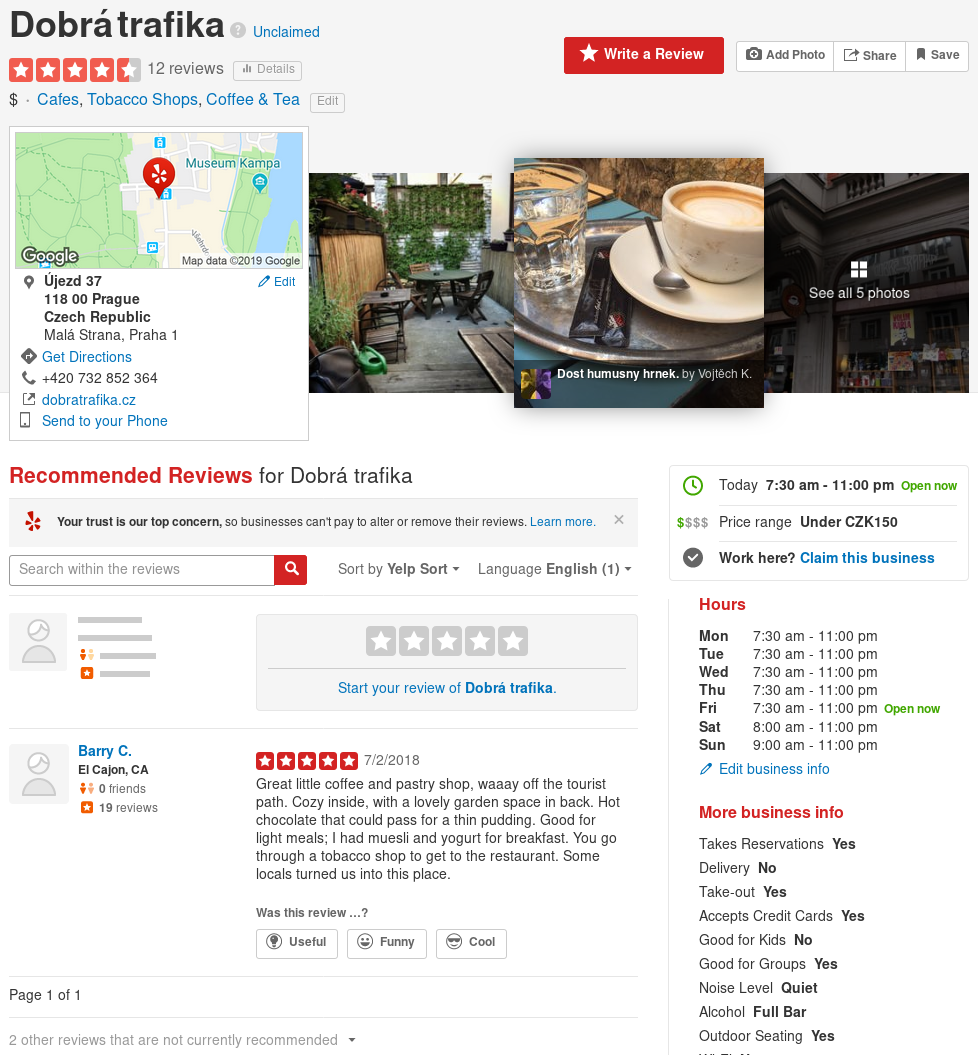
\includegraphics[width=130mm]{../img/dobra_trafika.png}
\caption{An example of an online profile}
\label{fig:dobra_trafika}
\end{figure}

A typical review of a restaurant looks like this:

\begin{code}
Charming decore. Delicious food. Friendly staff.
We'll certainly become repeat customers.
\end{code}

It contains unformatted pieces of information, fragments of sentences or typos.
In general, it can contain anything and \citet{Song14} define it as a new genre --- \textbf{short text}.
Short text is used in e-commerce systems and online communication in general.
It is usually up to 200 characters per document.
It is characterizes by its sparsity, free form and being large-scale and in the real time.
Although an average review in our data has 526 characters, we consider this short text.
First, it fulfills other characteristics.
Second, the bounds are not clearly defined.
An example of another short text system is Instant Messaging software Windows Live Messenger allowing up to 400 characters.

The reasons listed above make it difficult to work with short text.
Furthermore, there are many factors contributing to the difficulty of finding useful reviews.
First, we do not know the author and possibly have only a few reviews by the author.
Also, reviews by the same author can have different quality which is influenced by many factors,
such as the time spent on writing the review or whether the actual experience contains some useful information.
Therefore it is very hard to estimate author's reliability.
Second, reviews are very short, often containing only one piece of information.
Third, a review can quickly become obsolete or irrelevant.
Fourth, what is relevant to some, may not be to others.
All this also makes the task hard even for human operators and as such hard to evaluate our programme selecting useful reviews.

The main reason we chose Yelp is that users can flag properties of other reviews in the form of \emph{likes}.
Each review has three buttons --- \emph{useful}, \emph{funny} and \emph{cool} as can be seen in \Cref{fig:dobra_trafika}.
A user can vote for the property of a review by clicking on one of these buttons.
A typical review flagged as useful looks like this:

\begin{code}
A proper greasy spoon.
I was looking for a bacon flavoured hangover cure and I got one.
And a proper builders mug of tea.
Cheap as chips as well.
\end{code}

It clearly mentions the kind of the restaurant, what to seek there,
who it can be for and price.

On the other hand, a typical not-useful review looks like this:

\begin{code}
Awesome keg.. Always good, even with my own money!
\end{code}

It does only mention the place is good, but does not explain why --- price, friendly staff, location\dots.
The mention about money is unclear.
Does it mean the author has not got much money and therefore appreciate their cheap prices? Or something else?

Sometimes the review is not of a big quality itself, but contains some piece of information which makes it useful.
The review bellow is of a poor quality, not well formatted and only mentioning that we should not go there.
However, the mention about the bouncer and the tip turns out to be very useful for many users,
because it informs about the additional expenses added to the cost.

\begin{code}
Dont bother...this place is a dive!
The bouncer demanded a tip, just to seat us...def seek elsewhere...
you've been warned!!!
\end{code}

Of course, it is often near to impossible to decide whether a review is useful or not.
The review bellow clearly expresses pros and cons.
It is not a place to go when in hurry, not great for some delicious food,
but it is alright when we are not in hurry and want to have a friendly service.
However, the points are somewhat vague and the review is very subjective.

\begin{code}
It was OK. Service was friendly, but slow.
Food was OK, but I don't think it was a good value.
\end{code}


More about the data and the platform can be found in \Cref{app:dataset}.

Our objective is to create a software package that predicts whether some users would flag a restaurant review as a useful.
This prediction can be used for filtering out only useful reviews in a real review system.
We utilize means of supervised binary classification.
The useful likes are used for labelling reviews as \textit{useful} and \textit{not-useful}.
To ensure they have been viewed by enough users to get enough likes,
we take reviews only from a particular time frame
and we use only frequent restaurants with detailed profiles for the same reason.
We focus on classification of English reviews.

This is a well studied field and to date, many approaches to solve this have been introduced.
However, there is no clearly best performing algorithm for particular application.
Our main goal is therefore to compare already existing approaches.
The results can serve as a guide when implementing a real review system.

\section{Roadmap}

In \textbf{\Cref{chap:cls} Text Classification}, we define our task properly as text classification and briefly mention classification in different contexts.
We describe the utilized machine learning methods with examples of concrete usage.

In \textbf{\Cref{chap:fea} Feature Engineering}, we discuss several possibilities how to extract properties called features from text and how to filter only those useful.
Next, we mention dimension reduction as a possibility to reduce the complexity of our solution.
Finally, we introduce several commonly used features and filtering methods.
To a lessen degree, we also talk about non-textual data as well.

In \textbf{\Cref{chap:eval} Evaluation}, we introduce methods for comparing different algorithms.
We describe what requirements we expect a good algorithm to satisfy and how to use the data for comparing performance.
Lastly, we mention commonly used metrics to give us some easily comparable numbers.

In \textbf{\Cref{chap:arch} The Software Project Architecture}, we describe at the conceptual level our software package.
We describe individual modules, how they interact and the overall project structure.
We also talk about different files and configuration the project needs and commands used for running the project.

In \textbf{\Cref{chap:exp} Conducted Experiments}, we outline the experiments.
We describe combinations of algorithms we used and discuss the results.
We justify the compromises made for performance reasons.
Finally, we talk about the impact of size of the data to the performance.

In \textbf{\Cref{app:dataset} Yelp Dataset},
we describe the source of the data and its exact format.
We demonstrate how reviewing of businesses work and
the exact format of the data.

In \textbf{\Cref{app:prepr} Data Preprocessing},
we describe the challenge of obtaining reliable data and
what preprocessing has been done to allow easier manipulation and increase in reliability of the usefulness metrics.

In \textbf{\Cref{app:geneea} Geneea Data},
we describe the NLP analysis used for extracting sentiment and entities.

In \textbf{\Cref{app:techn} Package Technicalities},
we describe technical details and peculiarities of the software package.
We also provide commands for running the experiments and specify configuration.

In \textbf{\Cref{app:mi} Top Features by Mutual Information},
we list mutual information of selected features.


\section{Typographic Conventions}

In this thesis, we use the following typographic conventions:

\begin{itemize}
\item \textbf{bold} for definitions of new terms

\item \textit{italics} for mentions of already defined names. It also denotes data files in \Cref{chap:arch}.

\item \texttt{monospace} is used for code and filenames. It is used for process names in \Cref{chap:arch}.

\end{itemize}

\section{Related Work}

A lot of research has been done in short text classification.
Executive summary can be found in \citet{Song14}.
They define short text as a new genre; listing its characteristics, summarizing possible approaches to short text classification and evaluating performance.

One of the well studied dataset is tweets from Twitter.\footnote{\url{https://twitter.com}}
A lot of studies on sentiment analysis have been conducted.
\citet{jiang2011target} allege that most approaches follow
\citet{pang2002thumbs} who utilize machine learning based classifiers;
the state-of-the-art being \citet{go2009twitter} and \citet{barbosa2010robust}.
Perhaps more relevant study on Twitter is \citep{sriram2010short},
which tackles the problem of filtering relevant information.

Reviews are to author's knowledge less studied.
One of the relevant papers is \citet{ganu2009beyond}.
They discuss the difficulties of selecting useful restaurant reviews.
Unlike this thesis, they do not classify reviews as a whole, but instead try to find reviews containing topics such as food or service.
The main attempt is to find some structure in the free form.

Related text classification research focuses on sentiment analysis and toxic speech detection.
A lot of research is focusing on sentiment analysis.

Relatively close research focuses on toxic speech.
\citet{van2018challenges} talk about toxic speech as non-constructive and non-inclusive conversation including hate speech, threats, insults and in general fruitless conversation.
Filtering out fruitless text is our focus to high extent too.
Apart from already mentioned challenges they mention high variance in performance and difficulty to define the topic clearly.
Basic review of toxic speech classification can be found in \citet{gunasekara2018review}.

\chapter{Yelp Open Dataset}

Yelp is a US-based company whose goal is: ``to connect people with great local businesses.''\footnote{\url{https://yelp.com/about}}
It provides both mobile and web interface listing businesses such as restaurants or shopping centres.
Users can easily post a review for any business based on their recent visit.
All this makes the platform very popular and because of its convenience many people review businesses.

There are three main reasons we chose to evaluate our algorithms on this dataset.
As we mentioned this platform is very popular and as such has sufficient data.

Secondly, the company publishes every year an open dataset which can be downloaded for academic
purposes.
It covers most information conveyed in their system ---  information about businesses and users, pictures taken by the users and most importantly for us textual reviews.
As such it is possible to download the entire dataset without having to scrape some data.

Lastly, this dataset allows us to asses the needed properties of individual reviews.
The platform not only allows users to post reviews, but also to asses other reviews in form of \emph{likes}.
Each review has three buttons --- \emph{useful}, \emph{funny} and \emph{cool}.
A user can express the property of a review by clicking on one of these buttons. Information how many times these buttons have been clicked is also present in the dataset and as such makes it a great dataset for evaluating how well our algorithms perform.

\todoA{very brief mention about dataset format and link to appendix}

\chapter{Text Classification}

% \begin{tikzpicture}
%   \begin{scope}[blend group = soft light]
%     \fill[red!30!white]   ( 90:1.2) circle (2);
%     \fill[green!30!white] (210:1.2) circle (2);
%     \fill[blue!30!white]  (330:1.2) circle (2);
%   \end{scope}
%   \node at ( 90:2)    {Typography};
%   \node at ( 210:2)   {Design};
%   \node at ( 330:2)   {Coding};
%   \node [font=\Large] {\LaTeX};
% \end{tikzpicture}

The process of~selecting useful review is an example of {\bf text classification}.
\citet{AggZhai12} describe text classification as follows.
We have records~$X_1, \ldots, X_N$ and labels~$1,\ldots, k$.
Record is a standalone unit and is assigned one label.
Text classification aims to predict what label it is.

Every record consists of~attributes which convey some~information about it.
An example of an attribute is the text of a review or the number of stars given by the user.
We will refer to a~record as {\bf an~instance} to be consistent with machine learning terminology.
{\bf Text classification} is then a process of building a classification model that is able to assign
an instance its label based solely on its attributes.
{\bf Classification model} (also called classifier) is a~mapping between an~instance and a~class label.

\todoA{diagram records -> labels - records=instances; labels; arrows are the model}
	\begin{code}
		review            -->        useful

		review2		-->			not-useful


		review3 arrow up

		^^^^^^^						^^^^^
		instance					labels

		arrows = model
	\end{code}


As \citet{TanBachKum08} distinguish it, classification is either {\it descriptive} and {\it predictive}.
Descriptive is for finding regularities in data.
An example of descriptive classification is a task where
biologists try to figure out what the features distinguishing mammals and birds are.
In this thesis, we will consider only predictive classification, where the goal is to build a classifier
that can predict labels for new instances.

We have two sets of instances to be able to asses how well our model predicts instances.
First, a training set is  used for building a~classification model.
Second, a testing set is used for assessing how well the model predicts labels for new instances.
Because the testing set contains the actual labels, we can compare our predictions with them.

The approach of fitting a classifier to labelled data is called \textbf{supervised learning}.
We have the results of classification and we are trying to build a model that approximates these results.
On the contrary, \textbf{unsupervised learning} means that we do not know the labels and we try to group instances that are in some respect similar without having labels.

In~this thesis, we take into account only \textbf{hard version} of~classification which explicitly maps one and only one label to each record.  
\textbf{Soft version} assign probabilities to labels.

\section{Text Classification Process}

TODO - tady jsme skoncili - prepsat tohle neni hezke

The process of classification is broken down into four parts as shown in \autoref{fig:cls_process}.

\todoA{diagram:}
\begin{figure}
\begin{code}
obtaining dataset
-> preprocessing {extraction} -> feature selection
 ^^^^^^^^^^^^^^^^^^^^^^^^^^^^^^^^^^^^^^^^^^^^^^^^^^^^^^
    		feature engineering

-> training -> evaluation
\end{code}
	blah\label{fig:cls_process}
\end{figure}


We always need to obtain sufficient information about each instance.
This mean we can use more sources.
Obtaining data usually comprises of data scraping or otherwise downloading it.
We do not cover this, because the Yelp dataset is freely available for download.

We cannot feed the data directly into our classifier.
The data has to be preprocessed first.
This process is called {\bf feature engineering}.
We extract the so called {\bf features}, which carry some information about the instance.
Feature is simply some property of an instance like the number of words in a review.
As we will see, it is hard to come up with features that would directly lead to successful classification.
Hence, we will try to generate as many features as we can and then try to select the most useful.
We will discuss both feature extraction and selection in \autoref{chap:fea}.


Once the data is ready, we build a classifier from the preprocessed data.
This phase is called training.
Finally, we want to be able to compare different classifiers and feature sets.
Common evaluations will be discussed in \autoref{chap:eval}.

Last three chapters  are left for the architecture of the software developed (\autoref{chap:arch}),
demonstration of conducted experiments (\autoref{chap:exp}) and final discussion (\autoref{chap:concl}).



\section{\todoB{What a Classifier Looks Like}}

\todoB{Probabilistic model for classification
Generally speaking, there are two models used for classification; generative and discriminative. Generative model assumes there exist }

\subsection{\todoB{hyperparameteres, parameters, model}}

\subsection{\todoC{discrm. vs generative}}

\todoB{linear classifier def}

\section{Classifiers}
\label{chap:clscon}

As we mentioned, classification is a process of building a classification model which maps
instances onto labels.
In this section, we will describe some commonly used classifiers.
We will demonstrate them on mock data shown in \autoref{tab:custsatis}.
We have a fictional dataset of customers of a mobile carrier and
we are trying to predict whether customers are satisfied.
The rows are instances and columns features.
Our three features are 
whether the customer received a discount (yes or no), whether it is a private customer (yes or no)
and what mobile internet is part of their prepaid plan (none, limited and unlimited).
We are predicting the last column.

Please note that our primar focus is text classification.
However, we will use non-textual features in this example for easier understanding.
Classifiers (except for fastText which is tailored specifically for text) take any set of features,
so we can use them in the same way with features extracted directly from text.
We will learn how to do that in \autoref{chap:fea}.

\begin{table}[h!]

\centering
\begin{tabular}{lllll}
\toprule
\textbf{ID} & \textbf{discount} & \textbf{private} & \textbf{internet} \hspace{1.cm} & \textbf{satisfied} \\
\midrule
1 & yes & yes & unlimited & yes \\
2 & no & yes & unlimited & yes \\
3 & no & no & unlimited & no \\
4 & yes & yes & no & yes \\
5 & no & yes & limited & no \\
6 & yes & no & limited & yes \\
7 & no & yes & no & no \\
\bottomrule
\end{tabular}

\caption{Customer satisfaction example}\label{tab:custsatis}
\end{table}






\subsection{Zero-R, One-R}

These two algorithms are used as a baseline.
Baseline algorithm is a very simple method used to get better idea about the dataset and dificulty of our task.
It is useful to have a comparison to whatever more sophisticated we developed.
Suppose, we have a very sophisticated classifier predicting 22\% instances correctly
We may lean to say that the performance is not really good.
And if the baseline gets 20\% well, it may really be that case.
However, when our baseline predicts only 3\%, 22\% may be actually very good results worth the effort.

{\bf Zero-R} simply takes the most frequent label and labels every instance with it.
Zero-R would label all customers as satisfied in our example.

A bit more complicated {\bf One-R} chooses one feature and bases the classification solely on this feature.
For every value of the feature, we take all instances corresponding to this value and choose the label occurring the most among them.
For predicting, we use the label we found for each value.

Suppose we choose the feature {\it discount} in our example.
We can see that all customers that got discount are satisfied.
Hence all customers getting a discount are according to one-R satisfied.
Three customers that did not get discount are dissatisfied and one is satisfied.
Hence one-R will predict all customers without a discount as dissatisfied.

The problem is how to choose the most informative feature which we will tackle in \autoref{subsec:decisiontree}.
For now we can think of it as finding such a feature, that will produce the best classifier.

\subsection{Na\"{i}ve Bayes}

Na\"{i}ve Bayes is a probabilistic classifier.
Probabilistic means that we classify an instance according to the probabilities of the instance belonging to individual classes (having that label).
Mathematically speaking, we choose label~$\hat{c}$~from the set of all labels $C=\left\{c_1,c_2,\dots c_n\right\}$ for instance~$d_j$, such that:

\begin{equation}
	\label{eq:argmax}
	\hat{c} = \argmax_{c_i \in C} P\left(c_i  | d_j \right),
\end{equation}

where~$P\left(c_i | d_j\right)$~is the probability of~$d_j$~being labelled with~$c_i$.
Note that we use \textit{arg\,max} which equals to the value of the argument variable
with the highest value of the expression.

However, we do not directly say what label belongs to the instance we are predicting.
Instead, Na\"{i}ve Bayes uses the so-called generative model.
In generative model, we assume every instance is generated by a parametric model.
\textbf{Parametric model} consists of~$n$~components $c_1, c_2,\ldots, c_n$.
Every component corresponds to one class label
and is said to generate all instances with this label.
Note that since there is one-to-one correspondence between classes and components,
we use the same notation for both components and labels.
It should be clear from the context what we mean (i.e. component generates an instance,
but an instance is assigned a label).
Also note, that the assumption about class and component correspondence is only used for simplification and can be generalised \todoA{source}.

An instance is generated in two steps.
First, a component is selected according to priors.
Priors are the apriori probabilities of the current model denoted by $P\left(c_i\right)$ for component~$c_i$.
Second, an instance is generated by this component according to posterios.
Posteriors are probabilities of instance~$d_j$~being generated by component~$c_i$~denoted by~$P\left(d_j|c_i\right)$.

The likelihood of instance~$d_i$~being generated is then:

\begin{equation}
	P\left(d_j\right) = \sum_{i=1}^{n}{
	P\left(c_i\right)
	P\left(d_j|c_i\right)
}
\end{equation}

Next, we need to convert these probabilities into the probability of an instance having a label.
We can infer \autoref{eq:bayesrule} (called \textbf{Bayes rule}) from \autoref{eq:bayesinfer}.

\begin{equation}
	\label{eq:bayesinfer}
	P\left(A,B\right) = 
	P\left(A|B\right)
	P\left(B\right) = 
	P\left(A\right)
	P\left(B|A\right),
\end{equation}
\begin{equation}
	\label{eq:bayesrule}
	P\left(A|B\right) =
	\frac{
	P\left(A\right)
P\left(B|A\right)}
{P\left(B\right)}
\end{equation}

Our original \autoref{eq:argmax}

\begin{equation}
	\hat{c} = \argmax_{c_i \in C} P\left(c_i  | d_j \right)
\end{equation}

can be transcribed with Bayes rule as:

\begin{equation}
	\hat{c} = \argmax_{c_i \in C}
	\frac{
	P\left(d_j  | c_i \right)
	P\left( c_i \right)
}{
	P\left( d_j \right)
}
\end{equation}

Because we are not interested in the exact value of the expression, it is equivalent to:

\begin{equation}
	\label{eq:classprb}
	\hat{c} = \argmax_{c_i \in C}
	P\left(d_j  | c_i \right)
	P\left( c_i \right)
\end{equation}

The exact values of probabilities are calculated as follows.
Prior probabilities are the distribution of classes.
The exact values are computed by counts.
For computing posterios, Na\"{i}ve Bayes assumption is used.
It says that each feature is independent of all other features.
Note that in practical context, the assumption often does not hold.
However, since we are only interested in the label with highest probability,
not the probability itself, possible errors are often insignificant and Na\"{i}ve Bayes often works in practise even when the features are not independent.
Thanks to the assumption, the probability of an instance represented by feature values is the product
of probabilities of individual features having the given values.
For features $f_1, f_2, \dots f_K$ it is:

\begin{equation}
	\label{eq:posterios}
	P\left(d_j  | c_i \right) = \prod_{k=1}^{K}
	{P\left(  f_k  | c_i \right)}
\end{equation}

By combining \autoref{eq:classprb} and \autoref{eq:posterios}, we get:

\begin{equation}
	\hat{c} = \argmax_{c_i \in C}
	\prod_{k=1}^{K}
	{P\left(  f_k  | c_i \right)}
	P\left( c_i \right)
\end{equation}

Probability~$P\left(f_k|c_i\right)$~is found by counting.
We take all instances from class~$c_i$~and the probability is the ratio of all those instances with the same value of feature~$f_k$~and the rest.

Let us classify instance~$\mathit{ID}=2$~from our mock data in \autoref{tab:custsatis} for demonstration.
For label ``yes'' (satisfied customers):

\begin{equation}
	t_{yes} = 
	\prod_{k=1}^{K}
	{P\left(  f_k  | c_{yes} \right)}
	P\left( c_{yes} \right)
\end{equation}

\begin{equation}
	t_{yes} = 
	P\left(  f_{dis} = no | c_{yes} \right)
	P\left(  f_{priv} = yes | c_{yes} \right)
	P\left(  f_{int} = unlim | c_{yes} \right)
	P\left( c_{yes} \right)
\end{equation}

$P\left(  f_{dis} = no | c_{yes} \right)$ equals $\frac{1}{4}$, because there are four satisfied customers
and only one of them did not receive discount.
Analogously, the remaining values are computed.
$P\left( c_{yes} \right)$ is $\frac{4}{7}$, because there are four satisfied customers out of seven.
Together we get:

\begin{equation}
	t_{yes} = 
	\frac{1}{4} \times
	\frac{3}{4} \times
	\frac{2}{4} \times
	\frac{4}{7}
	\sim 0.054
\end{equation}

We compute~$t_{no}$~in the same manner for a dissatisfied customer:

\begin{equation}
	t_{no} = 
	\prod_{k=1}^{K}
	{P\left(  f_k  | c_{no} \right)}
	P\left( c_{no} \right)
\end{equation}

\begin{equation}
	t_{no} = 
	P\left(  f_{dis} = no | c_{no} \right)
	P\left(  f_{priv} = no | c_{no} \right)
	P\left(  f_{int} = unlim | c_{no} \right)
	P\left( c_{no} \right)
\end{equation}

\begin{equation}
	t_{no} = 
	\frac{3}{3} \times
	\frac{2}{3} \times
	\frac{1}{3} \times
	\frac{3}{7}
	\sim 0.095
\end{equation}

$t_{no}$ is higher and Na\"{i}ve Bayes classifies the instance as dissatisfied.
Note that this may look surprising as features ``private'' and ``internet'' suggest satisfaction,
but the correlation between discount and satisfaction is so strong that it outweights other features in this settings.

\todoC{zminka prior a posterior ohledne maximizace je prave pocitani}



\subsection{Decision trees}
\label{subsec:decisiontree}
\todoC{Decision trees - if you decide not to do it, change ONE-R reference to evaluation}

\subsection{FastText}

FastText\footnote{\url{https://fasttext.cc}} is a small library developed by Facebook.
Text classification in this library is on par with current state-of-the-art deep learning classifiers
and many orders of magnitude faster~\citep{Joulin2017bag}.

Let us first explain a baseline algorithm on top of which fastText builds.
It uses {\it bag of words}\footnote{more on this in the subsection~\ref{subsec:bow}} as features.
This means that each instance is represented by a vector of numbers.
Every position in the vector corresponds to a particular word in a dictionary.
The value of the position denotes number of occurrences of the words in the instance.
A linear classifiers is trained on this.
Linear in this context means that the decision on classification is based on a linear combination of features.
Thanks to this, linear models are a lot faster than complicated neural networks, however the classification may not be as good.

FastText uses {\it word embeddings}\footnote{see the subsection~\ref{subsec:wordembed}} instead of a simple bag of words.
In short, it maps every word onto a vector. Every document is represented as an average vector of all words.

However, fastText goes even further.
The process is precisely described in \citet{Bojanowski2017enriching}.
we will only briefly summarize it.
Fasttext maps n-grams onto vectors, not words.
{\bf N-gram} is any sequence of n elements --- in this case letters.
The algorithm represents a words as an average of vectors of all its n-grams.
Let~$w_{a}$~be a vector representation of an n-gram~$a$, then 
the representation of \texttt{where} is the average of vectors
$w_{whe}$, 
$w_{her}$ and
$w_{ere}$.

For even higher performance, every word is surrounded by \texttt{<} and \texttt{>}.
The word \textit{ where} thus becomes \texttt{<where>}.
The vector of \texttt{where} becomes the average of vectors
$w_{<wh}$, 
$w_{whe}$, 
$w_{her}$,
$w_{ere}$ and
$w_{er>}$.
Note that trigram {\tt her} from \texttt{<where>} is different from {\tt <her} from the word {\tt <here>}.
It allows even better performance, because it distinguishes n-grams at the word boundaries and in the middle.

This approach has a few advantages.
Even words that are not seen during the training phase can be given a vector.
This is especially useful for languages with large vocabularies and many rare words.
Also, unlike the baseline approach, it covers the internal structure of words.
It is useful for morphologically rich languages such as Finnish or Turkish.
Finish has 15 different cases for nouns.
Many of which may not appear in the training set at all.
Hence being able to reasonably represent even unseen words is a big advantage,
because many words follow word formation rules which can be captured in n-grams.
Other implementations represent unseen words with some kind of dummy vector.

As we mentioned, every instance is average of vectors of its words.
This representation is used for training a simple linear classifier.
FastText uses some more tricks to reduce memory consumption and performance.
More details can be found in~\citet{Joulin2017bag}.

\todoA{a budeme muset pridat linearni model - pridej zminku o tom, jak se to klasifikuje podle toho, jestli nekde popises linearni modely vice}

\todoC{hierarchichal softmax}

\subsubsection{\todoC{GloVe - GloVe nepouzivam}}

\subsection{\todoC{NN}}

\subsection{\todoC{Let you imagination go wild}}


\section{\todoB{interpretability -see w8}}

%%% Fiktivní kapitola s ukázkami sazby

\chapter{Nápověda k~sazbě}

\section{Úprava práce}

Vlastní text bakalářské práce je uspořádaný hierarchicky do kapitol a podkapitol,
každá kapitola začíná na nové straně. Text je zarovnán do bloku. Nový odstavec
se obvykle odděluje malou vertikální mezerou a odsazením prvního řádku. Grafická
úprava má být v~celém textu jednotná.

Práce se tiskne na bílý papír formátu A4. Okraje musí ponechat dost místa na vazbu:
doporučen je horní, dolní a pravý okraj $25\,\rm mm$, levý okraj $40\,\rm mm$.
Číslují se všechny strany kromě obálky a informačních stran na začátku práce;
první číslovaná strana bývá obvykle ta s~obsahem.

Písmo se doporučuje dvanáctibodové ($12\,\rm pt$) se standardní vzdáleností mezi řádky
(pokud píšete ve Wordu nebo podobném programu, odpovídá tomu řádkování $1,5$; v~\TeX{}u
není potřeba nic přepínat). Pro běžný text používejte vzpřímené patkové písmo.
Text matematických vět se obvykle tiskne pro zdůraznění skloněným (slanted) písmem,
není-li k~dispozici, může být zastoupeno kurzívou.

Primárně je doporučován jednostranný tisk (příliš tenkou práci lze obtížně svázat).
Delší práce je lepší tisknout oboustranně a přizpůsobit tomu velikosti okrajů:
$40\,\rm mm$ má vždy \emph{vnitřní} okraj. Rub titulního listu zůstává nepotištěný.

Zkratky použité v textu musí být vysvětleny vždy u prvního výskytu zkratky (v~závorce nebo
v poznámce pod čarou, jde-li o složitější vysvětlení pojmu či zkratky). Pokud je zkratek
více, připojuje se seznam použitých zkratek, včetně jejich vysvětlení a/nebo odkazů
na definici.

Delší převzatý text jiného autora je nutné vymezit uvozovkami nebo jinak vyznačit a řádně
citovat.

\section{Jednoduché příklady}

Čísla v~českém textu obvykle sázíme v~matematickém režimu s~desetinnou čárkou:
%%% Bez \usepackage{icomma}:
% $\pi \doteq 3{,}141\,592\,653\,589$.
%%% S \usepackage{icomma}:
$\pi \doteq 3,141\,592\,653\,589$.
V~matematických textech se považuje za přípustné používat desetinnou tečku
(pro lepší odlišení od čárky v~roli oddělovače). Numerické výsledky se uvádějí
s~přiměřeným počtem desetinných míst.

Mezi číslo a jednotku patří úzká mezera: šířka stránky A4 činí $210\,\rm mm$, což si
pamatuje pouze $5\,\%$ autorů. Pokud ale údaj slouží jako přívlastek, mezeru vynecháváme:
$25\rm mm$ okraj, $95\%$ interval spolehlivosti.

Rozlišujeme různé druhy pomlček:
červeno-černý (krátká pomlčka),
strana 16--22 (střední),
$45-44$ (matematické minus),
a~toto je --- jak se asi dalo čekat --- vložená věta ohraničená dlouhými pomlčkami.

V~českém textu se používají \uv{české} uvozovky, nikoliv ``anglické''.

% V tomto odstavci se vlnka zviditelňuje
{
\def~{{\tt\char126}}
Na některých místech je potřeba zabránit lámání řádku (v~\TeX{}u značíme vlnovkou):
u~předložek (neslabičnych, nebo obecně jednopísmenných), vrchol~$v$, před $k$~kroky,
a~proto, \dots{} obecně kdekoliv, kde by při rozlomení čtenář \uv{ško\-brt\-nul}.
}

\section{Matematické vzorce a výrazy}

Proměnné sázíme kurzívou (to \TeX{} v~matematickém módu dělá sám, ale
nezapomínejte na to v~okolním textu a také si matematický mód zapněte).
Názvy funkcí sázíme vzpřímeně. Tedy například:
$\var(X) = \E X^2 - \bigl(\E X \bigr)^2$.

Zlomky uvnitř odstavce (třeba $\frac{5}{7}$ nebo $\frac{x+y}{2}$) mohou
být příliš stísněné, takže je lepší sázet jednoduché zlomky s~lomítkem:
$5/7$, $(x+y)/2$.

Nechť
\[   % LaTeXová náhrada klasického TeXového $$
\mathbb{X} = \begin{pmatrix}
      \T{\bm x_1} \\
      \vdots \\
      \T{\bm x_n}
      \end{pmatrix}.
\]
Povšimněme si tečky za~maticí. Byť je matematický text vysázen
ve~specifickém prostředí, stále je gramaticky součástí věty a~tudíž je
zapotřebí neopomenout patřičná interpunkční znaménka. Výrazy, na které
chceme později odkazovat, je vhodné očíslovat:
\begin{equation}\label{eq01:Xmat}
\mathbb{X} = \begin{pmatrix}
      \T{\bm x_1} \\
      \vdots \\
      \T{\bm x_n}
      \end{pmatrix}.
\end{equation}
Výraz \eqref{eq01:Xmat} definuje matici $\mathbb{X}$. Pro lepší čitelnost
a~přehlednost textu je vhodné číslovat pouze ty výrazy, na které se
autor někde v~další části textu odkazuje. To jest, nečíslujte
automaticky všechny výrazy vysázené některým z~matematických
prostředí.

Zarovnání vzorců do několika sloupečků:
\begin{alignat*}{3}
S(t) &= \pr(T > t),    &\qquad t&>0       &\qquad&\text{ (zprava spojitá),}\\
F(t) &= \pr(T \leq t), &\qquad t&>0       &\qquad&\text{ (zprava spojitá).}
\end{alignat*}

Dva vzorce se spojovníkem:
\begin{equation}\label{eq01:FS}
\left.
\begin{aligned}
S(t) &= \pr(T > t) \\[1ex]
F(t) &= \pr(T \leq t)
\end{aligned}
\;	% zde pomůže ručně vynechat trochu místa
\right\}
\quad t>0 \qquad \text{(zprava spojité).}
\end{equation}

Dva centrované nečíslované vzorce:
\begin{gather*}
\bm Y = \mathbb{X}\bm\beta + \bm\varepsilon, \\[1ex]
\mathbb{X} = \begin{pmatrix} 1 & \T{\bm x_1} \\ \vdots & \vdots \\ 1 &
  \T{\bm x_n} \end{pmatrix}.
\end{gather*}
Dva centrované číslované vzorce:
\begin{gather}
\bm Y = \mathbb{X}\bm\beta + \bm\varepsilon, \label{eq02:Y}\\[1ex]
\mathbb{X} = \begin{pmatrix} 1 & \T{\bm x_1} \label{eq03:X}\\ \vdots & \vdots \\ 1 &
  \T{\bm x_n} \end{pmatrix}.
\end{gather}

Definice rozdělená na dva případy:
\[
P_{r-j}=
\begin{cases}
0, & \text{je-li $r-j$ liché},\\
r!\,(-1)^{(r-j)/2}, & \text{je-li $r-j$ sudé}.
\end{cases}
\]
Všimněte si použití interpunkce v této konstrukci. Čárky a tečky se
dávají na místa, kam podle jazykových pravidel patří.

\begin{align}
x& = y_1-y_2+y_3-y_5+y_8-\dots = && \text{z \eqref{eq02:Y}} \nonumber\\
& = y'\circ y^* = && \text{podle \eqref{eq03:X}} \nonumber\\
& = y(0) y' && \text {z Axiomu 1.}
\end{align}


Dva zarovnané vzorce nečíslované:
\begin{align*}
L(\bm\theta) &= \prod_{i=1}^n f_i(y_i;\,\bm\theta), \\
\ell(\bm\theta) &= \log\bigl\{L(\bm\theta)\bigr\} =
\sum_{i=1}^n \log\bigl\{f_i(y_i;\,\bm\theta)\bigr\}.
\end{align*}
Dva zarovnané vzorce, první číslovaný:
\begin{align}
L(\bm\theta) &= \prod_{i=1}^n f_i(y_i;\,\bm\theta), \label{eq01:L} \\
\ell(\bm\theta) &= \log\bigl\{L(\bm\theta)\bigr\} =
\sum_{i=1}^n \log\bigl\{f_i(y_i;\,\bm\theta)\bigr\}. \nonumber
\end{align}

Vzorec na dva řádky, první řádek zarovnaný vlevo, druhý vpravo, nečíslovaný:
\begin{multline*}
\ell(\mu,\,\sigma^2) = \log\bigl\{L(\mu,\,\sigma^2)\bigr\} =
\sum_{i=1}^n \log\bigl\{f_i(y_i;\,\mu,\,\sigma^2)\bigr\}= \\
  = -\,\frac{n}{2}\,\log(2\pi\sigma^2) \,-\,
\frac{1}{2\sigma^2}\sum_{i=1}^n\,(y_i - \mu)^2.
\end{multline*}

Vzorec na dva řádky, zarovnaný na $=$, číslovaný uprostřed:
\begin{equation}\label{eq01:ell}
\begin{split}
\ell(\mu,\,\sigma^2) &= \log\bigl\{L(\mu,\,\sigma^2)\bigr\} =
\sum_{i=1}^n \log\bigl\{f(y_i;\,\mu,\,\sigma^2)\bigr\}= \\
& = -\,\frac{n}{2}\,\log(2\pi\sigma^2) \,-\,
\frac{1}{2\sigma^2}\sum_{i=1}^n\,(y_i - \mu)^2.
\end{split}
\end{equation}

\section{Definice, věty, důkazy, \dots}

Konstrukce typu definice, věta, důkaz, příklad, \dots je vhodné
odlišit od okolního textu a~případně též číslovat s~možností použití
křížových odkazů. Pro každý typ těchto konstrukcí je vhodné mít
v~souboru s~makry (\texttt{makra.tex}) nadefinované jedno prostředí,
které zajistí jak vizuální odlišení od okolního textu, tak
automatické číslování s~možností křížově odkazovat.

\begin{definice}\label{def01:1}
  Nechť náhodné veličiny $X_1,\dots,X_n$ jsou definovány na témž
  prav\-dě\-po\-dob\-nost\-ním prostoru $(\Omega,\,\mathcal{A},\,\pr)$. Pak
  vektor $\bm X = \T{(X_1,\dots,X_n)}$ nazveme \emph{náhodným
    vektorem}.
\end{definice}

\begin{definice}[náhodný vektor]\label{def01:2}
  Nechť náhodné veličiny $X_1,\dots,X_n$ jsou definovány na témž
  pravděpodobnostním prostoru $(\Omega,\,\mathcal{A},\,\pr)$. Pak
  vektor $\bm X = \T{(X_1,\dots,X_n)}$ nazveme \emph{náhodným
    vektorem}.
\end{definice}
Definice~\ref{def01:1} ukazuje použití prostředí pro sazbu definice
bez titulku, definice~\ref{def01:2} ukazuje použití prostředí pro
sazbu definice s~titulkem.

\begin{veta}\label{veta01:1}
  Náhodný vektor $\bm X$ je měřitelné zobrazení prostoru
  $(\Omega,\,\mathcal{A},\,\pr)$ do $(\R_n,\,\mathcal{B}_n)$.
\end{veta}

\begin{lemma}[\citealp{Andel07}, str. 29]\label{veta01:2}
  Náhodný vektor $\bm X$ je měřitelné zobrazení prostoru
  $(\Omega,\,\mathcal{A},\,\pr)$ do $(\R_n,\,\mathcal{B}_n)$.
\end{lemma}
\begin{dukaz}
  Jednotlivé kroky důkazu jsou podrobně popsány v~práci \citet[str.
  29]{Andel07}.
\end{dukaz}
Věta~\ref{veta01:1} ukazuje použití prostředí pro sazbu matematické
věty bez titulku, lemma~\ref{veta01:2} ukazuje použití prostředí pro
sazbu matematické věty s~titulkem. Lemmata byla zavedena v~hlavním
souboru tak, že sdílejí číslování s~větami.

%%% Fiktivní kapitola s ukázkami citací

\chapter{Odkazy na literaturu}

Odkazy na literaturu vytváříme nejlépe pomocí příkazů
\verb|\citet|, \verb|\citep| atp.
(viz {\LaTeX}ový balíček \textsf{natbib}) a~následného použití
Bib{\TeX}u. V~matematickém textu obvykle odkazujeme stylem \uv{Jméno
autora/autorů (rok vydání)}, resp. \uv{Jméno autora/autorů [číslo
odkazu]}. V~českém/slovenském textu je potřeba se navíc vypořádat
s~nutností skloňovat jméno autora, respektive přechylovat jméno
autorky. Je potřeba mít na paměti, že standardní příkazy
\verb|\citet|, \verb|\citep|
produkují referenci se jménem autora/autorů v~prvním pádě a~jména
autorek jsou nepřechýlena.

Pokud nepoužíváme bib\TeX{}, řídíme se normou ISO 690 a zvyklostmi
oboru.

Jména časopisů lze uvádět zkráceně, ale pouze v~kodifikované podobě.

\section{Několik ukázek}

Mezi nejvíce citované statistické články patří práce Kaplana a~Meiera a~Coxe
\citep{KaplanMeier58, Cox72}. \citet{Student08} napsal článek o~t-testu.

Prof. Anděl je autorem učebnice matematické statistiky
\citep[viz][]{Andel98}. Teorii odhadu se věnuje práce
\citet{LehmannCasella98}. V~případě odkazů na specifickou informaci
(definice, důkaz, \dots) uvedenou v~knize bývá užitečné uvést
specificky číslo kapitoly, číslo věty atp. obsahující požadovanou
informaci, např. viz \citet[Věta 4.22]{Andel07} nebo \citep[viz][Věta
4.22]{Andel07}.

Mnoho článků je výsledkem spolupráce celé řady osob. Při odkazování
v~textu na článek se třemi autory obvykle při prvním výskytu uvedeme
plný seznam: \citet*{DempsterLairdRubin77} představili koncept EM
algoritmu. Respektive: Koncept EM algoritmu byl představen v~práci
Dempstera, Lairdové a~Rubina \citep*{DempsterLairdRubin77}. Při každém
dalším výskytu již používáme zkrácenou verzi:
\citet{DempsterLairdRubin77} nabízejí též několik příkladů použití EM
algoritmu. Respektive: Několik příkladů použití EM algoritmu lze
nalézt též v~práci Dempstera a~kol. \citep{DempsterLairdRubin77}.

U~článku s~více než třemi autory odkazujeme vždy zkrácenou formou:
První výsledky projektu ACCEPT jsou uvedeny v~práci Genbergové a~kol.
\citep{Genberget08}. V~textu \emph{nenapíšeme}: První výsledky
projektu ACCEPT jsou uvedeny v~práci \citet*{Genberget08}.

%%% Fiktivní kapitola s ukázkami tabulek, obrázků a kódu

\chapter{Tabulky, obrázky, programy}

Používání tabulek a grafů v~odborném textu má některá společná
pravidla a~některá specifická. Tabulky a grafy neuvádíme přímo do
textu, ale umístíme je buď na samostatné stránky nebo na vyhrazené
místo v~horní nebo dolní části běžných stránek. \LaTeX\ se o~umístění
plovoucích grafů a tabulek postará automaticky.

Každý graf a tabulku
očíslujeme a umístíme pod ně legendu. Legenda má popisovat obsah grafu
či tabulky tak podrobně, aby jim čtenář rozuměl bez důkladného
studování textu práce.

Na každou tabulku a graf musí být v~textu odkaz
pomocí jejich čísla. Na příslušném místě textu pak shrneme ty
nejdůležitější závěry, které lze z~tabulky či grafu učinit. Text by
měl být čitelný a srozumitelný i~bez prohlížení tabulek a grafů a
tabulky a grafy by měly být srozumitelné i~bez podrobné četby textu.

Na tabulky a grafy odkazujeme pokud možno nepřímo v~průběhu běžného
toku textu; místo \emph{\uv{Tabulka~\ref{tab03:Nejaka} ukazuje, že
    muži jsou v~průměru o~$9,9\,\rm kg$ těžší než ženy}} raději napíšeme
\emph{\uv{Muži jsou o~$9,9\,\rm kg$ těžší než ženy (viz
    Tabulka~\ref{tab03:Nejaka})}}.

\section{Tabulky}

\begin{table}[b!]

\centering
%%% Tabulka používá následující balíčky:
%%%   - booktabs (\toprule, \midrule, \bottomrule)
%%%   - dcolumn (typ sloupce D: vycentrovaná čísla zarovnaná na
%%%     desetinnou čárku
%%%     Všimněte si, že ve zdrojovém kódu jsou desetinné tečky, ale
%%%     tisknou se čárky.
%%% Dále používáme příkazy \pulrad a \mc definované v makra.tex

\begin{tabular}{l@{\hspace{1.5cm}}D{.}{,}{3.2}D{.}{,}{1.2}D{.}{,}{2.3}}
\toprule
 & \mc{} & \mc{\textbf{Směrod.}} & \mc{} \\
\pulrad{\textbf{Efekt}} & \mc{\pulrad{\textbf{Odhad}}} & \mc{\textbf{chyba}$^a$} &
\mc{\pulrad{\textbf{P-hodnota}}} \\
\midrule
Abs. člen     & -10.01 & 1.01 & \mc{---} \\
Pohlaví (muž) & 9.89   & 5.98 & 0.098 \\
Výška (cm)    & 0.78   & 0.12 & <0.001 \\
\bottomrule
\multicolumn{4}{l}{\footnotesize \textit{Pozn:}
$^a$ Směrodatná chyba odhadu metodou Monte Carlo.}
\end{tabular}

\caption{Maximálně věrohodné odhady v~modelu M.}\label{tab03:Nejaka}

\end{table}

U~\textbf{tabulek} se doporučuje dodržovat následující pravidla:

\begin{itemize} %% nebo compactitem z balíku paralist
\item Vyhýbat se svislým linkám. Silnějšími vodorovnými linkami
  oddělit tabulku od okolního textu včetně legendy, slabšími
  vodorovnými linkami oddělovat záhlaví sloupců od těla tabulky a
  jednotlivé části tabulky mezi sebou. V~\LaTeX u tuto podobu tabulek
  implementuje balík \texttt{booktabs}. Chceme-li výrazněji oddělit
  některé sloupce od jiných, vložíme mezi ně větší mezeru.
\item Neměnit typ, formát a význam obsahu políček v~tomtéž sloupci
  (není dobré do téhož sloupce zapisovat tu průměr, onde procenta).
\item Neopakovat tentýž obsah políček mnohokrát za sebou. Máme-li
  sloupec \textit{Rozptyl}, který v~prvních deseti řádcích obsahuje
  hodnotu $0,5$ a v~druhých deseti řádcích hodnotu $1,5$, pak tento
  sloupec raději zrušíme a vyřešíme to jinak. Například můžeme tabulku
  rozdělit na dvě nebo do ní vložit popisné řádky, které informují
o~nějaké proměnné hodnotě opakující se v~následujícím oddíle tabulky
  (např. \emph{\uv{Rozptyl${}=0,5$}} a níže \emph{\uv{Rozptyl${}=
      1,5$}}).
\item Čísla v~tabulce zarovnávat na desetinnou čárku.
\item V~tabulce je někdy potřebné používat zkratky, které se jinde
nevyskytují. Tyto zkratky můžeme vysvětlit v~legendě nebo
v~poznámkách pod tabulkou. Poznámky pod tabulkou můžeme využít i
k~podrobnějšímu vysvětlení významu  některých sloupců nebo hodnot.
\end{itemize}

\section{Obrázky}

Několik rad týkajících se obrázků a grafů.

\begin{itemize}
\item Graf by měl být vytvořen ve velikosti, v~níž bude použit
  v~práci. Zmenšení příliš velkého grafu vede ke špatné čitelnosti
  popisků.
\item Osy grafu musí být řádně popsány ve stejném jazyce, v~jakém je
  psána práce (absenci diakritiky lze tolerovat). Kreslíme-li graf
  hmotnosti proti výšce, nenecháme na nich popisky \texttt{ht} a
  \texttt{wt}, ale osy popíšeme \emph{Výška [cm]} a~\emph{Hmotnost
    [kg]}. Kreslíme-li graf funkce $h(x)$, popíšeme osy $x$ a $h(x)$.
  Každá osa musí mít jasně určenou škálu.
\item Chceme-li na dvourozměrném grafu vyznačit velké množství bodů,
  dáme pozor, aby se neslily do jednolité černé tmy. Je-li bodů mnoho,
  zmenšíme velikost symbolu, kterým je vykreslujeme, anebo vybereme
  jen malou část bodů, kterou do grafu zaneseme. Grafy, které obsahují
  tisíce bodů, dělají problémy hlavně v~elektronických dokumentech,
  protože výrazně zvětšují velikost souborů.
\item Budeme-li práci tisknout černobíle, vyhneme se používání barev.
  Čáry roz\-li\-šu\-je\-me typem (plná, tečkovaná, čerchovaná,\ldots), plochy
  dostatečně roz\-díl\-ný\-mi intensitami šedé nebo šrafováním. Význam
  jednotlivých typů čar a~ploch vysvětlíme buď v~textové legendě ke
  grafu anebo v~grafické legendě, která je přímo součástí obrázku.
\item Vyhýbejte se bitmapovým obrázkům o~nízkém rozlišení a zejména
  JPEGům (zuby a kompresní artefakty nevypadají na papíře pěkně).
  Lepší je vytvářet obrázky vektorově a vložit do textu jako PDF.
\end{itemize}

\section{Programy}

Algoritmy, výpisy programů a popis interakce s~programy je vhodné
odlišit od ostatního textu. Jednou z~možností je použití {\LaTeX}o\-vé\-ho balíčku
\texttt{fancyvrb} (fancy verbatim), pomocí něhož je v~souboru \texttt{makra.tex}
nadefinováno prostředí \texttt{code}. Pomocí něho lze vytvořit
např. následující ukázky.

\begin{code}
> mean(x)
[1] 158.90
> objekt$prumer
[1] 158.90
\end{code}
%$
Menší písmo:
\begin{code}[fontsize=\footnotesize]
> mean(x)
[1] 158.90
> objekt$prumer
[1] 158.90
\end{code}
%$
Bez rámečku:
\begin{code}[frame=none]
> mean(x)
[1] 158.90
> objekt$prumer
[1] 158.90
\end{code}
%$
Užší rámeček:
\begin{code}[xrightmargin=20em]
> mean(x)
[1] 158.90
> objekt$prumer
[1] 158.90
\end{code}
%$

\begin{figure}[p]\centering
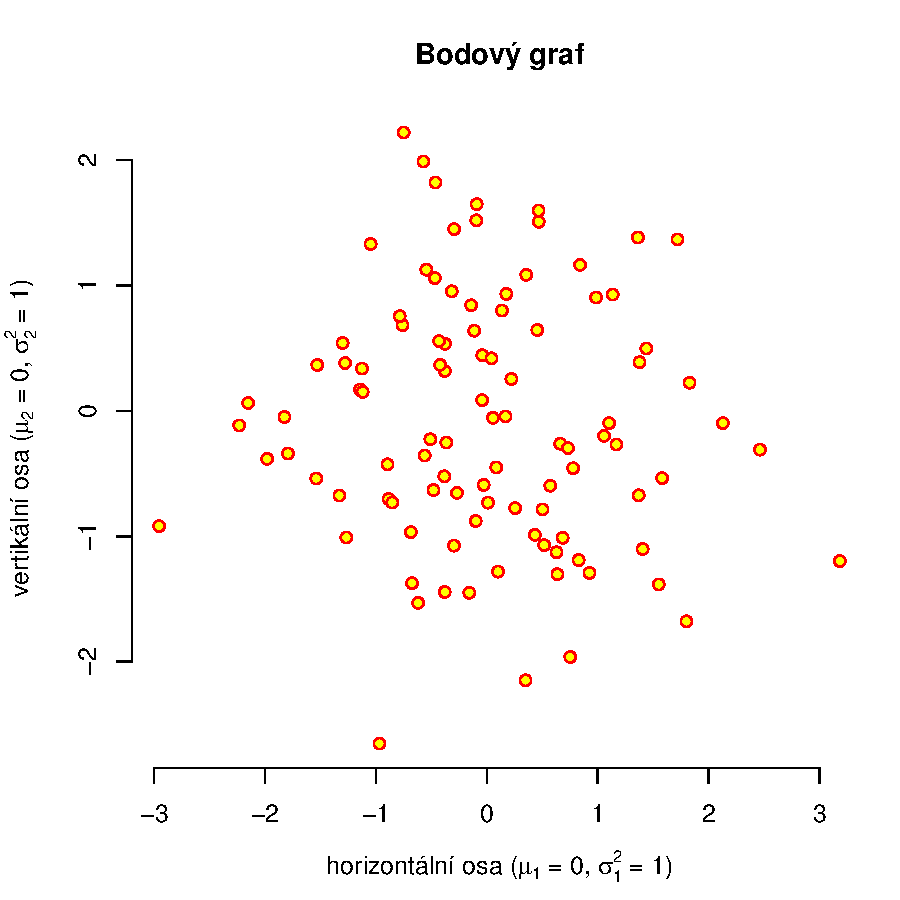
\includegraphics[width=140mm, height=140mm]{../img/ukazka-obr01}
% Příponu není potřeba explicitně uvádět, pdflatex automaticky hledá pdf.
% Rozměry také není nutné uvádět.
\caption{Náhodný výběr z~rozdělení $\mathcal{N}_2(\boldsymbol{0},\,I)$.}
\label{obr03:Nvyber}

\end{figure}

\begin{figure}[p]\centering
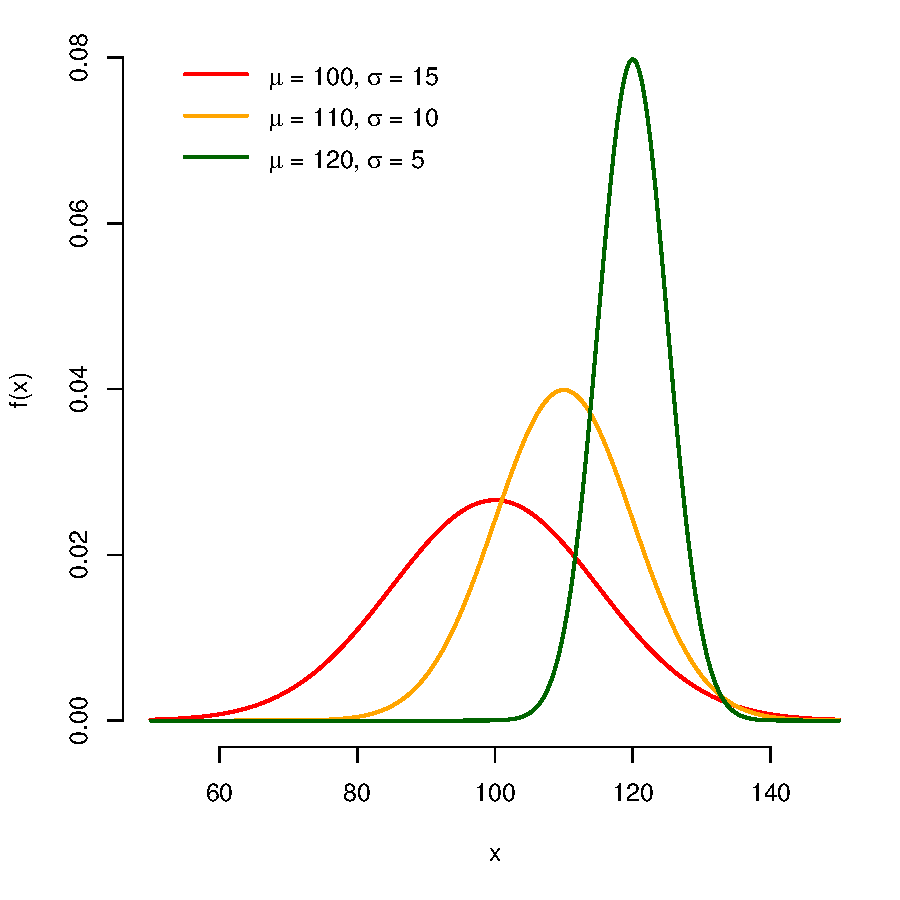
\includegraphics[width=140mm, height=140mm]{../img/ukazka-obr02}
\caption{Hustoty několika normálních rozdělení.}
\label{obr03:Nhust}
\end{figure}

\begin{figure}[p]\centering
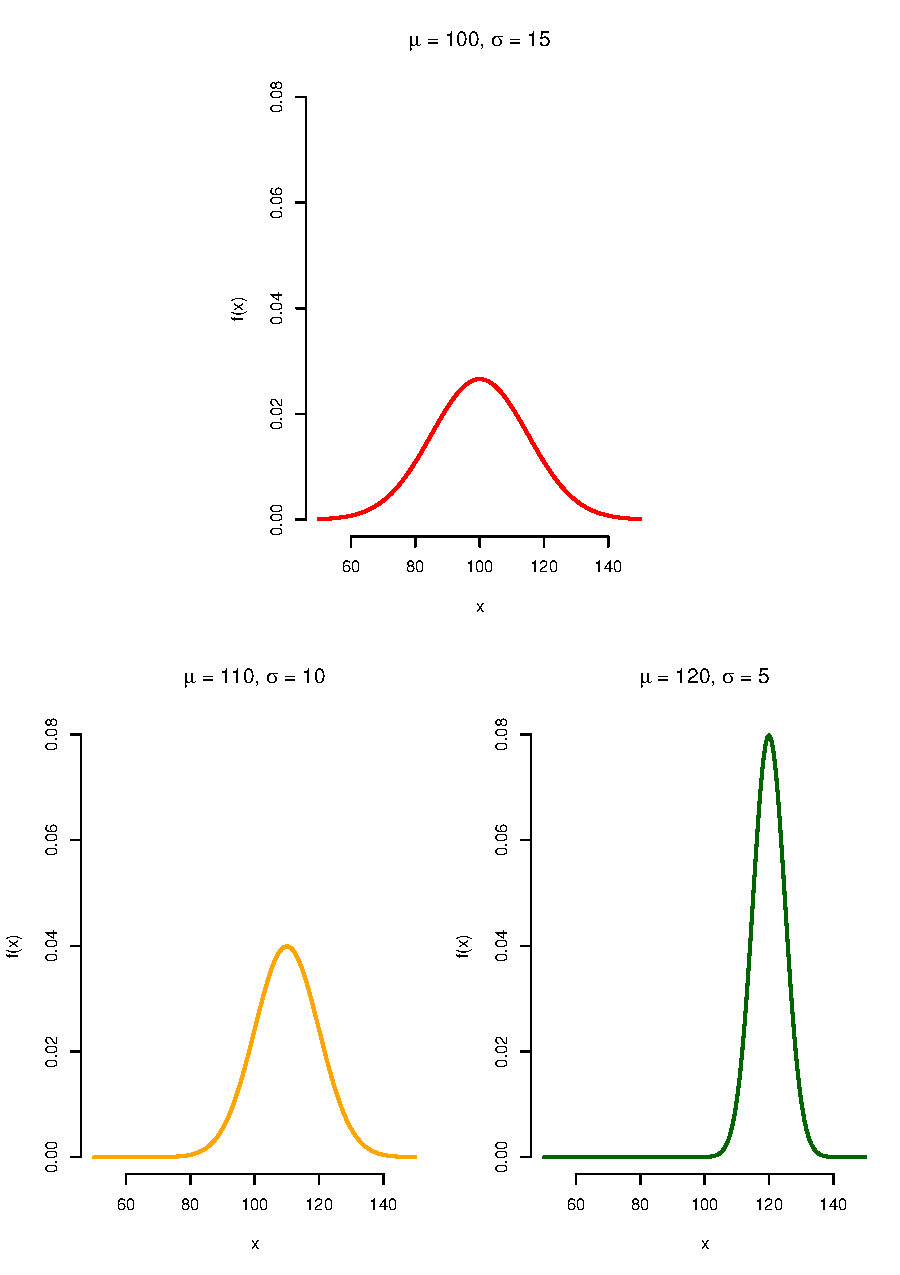
\includegraphics[width=140mm, height=198mm]{../img/ukazka-obr03}
\caption{Hustoty několika normálních rozdělení.}
\label{obr03:Nhust:podruhe}

\end{figure}

%%% Fiktivní kapitola s instrukcemi k PDF/A

\chapter{Formát PDF/A}

Opatření rektora č. 13/2017 určuje, že elektronická podoba závěrečných
prací musí být odevzdávána ve formátu PDF/A úrovně 1a nebo 2u. To jsou
profily formátu PDF určující, jaké vlastnosti PDF je povoleno používat,
aby byly dokumenty vhodné k~dlouhodobé archivaci a dalšímu automatickému
zpracování. Dále se budeme zabývat úrovní 2u, kterou sázíme \TeX{}em.

Mezi nejdůležitější požadavky PDF/A-2u patří:

\begin{itemize}

\item Všechny fonty musí být zabudovány uvnitř dokumentu. Nejsou přípustné
odkazy na externí fonty (ani na \uv{systémové}, jako je Helvetica nebo Times).

\item Fonty musí obsahovat tabulku ToUnicode, která definuje převod z~kódování
znaků použitého uvnitř fontu to Unicode. Díky tomu je možné z~dokumentu
spolehlivě extrahovat text.

\item Dokument musí obsahovat metadata ve formátu XMP a je-li barevný,
pak také formální specifikaci barevného prostoru.

\end{itemize}

Tato šablona používá balíček {\tt pdfx,} který umí \LaTeX{} nastavit tak,
aby požadavky PDF/A splňoval. Metadata v~XMP se generují automaticky podle
informací v~souboru {\tt prace.xmpdata} (na vygenerovaný soubor se můžete
podívat v~{\tt pdfa.xmpi}).

Validitu PDF/A můžete zkontrolovat pomocí nástroje VeraPDF, který je
k~dispozici na \url{http://verapdf.org/}.

Pokud soubor nebude validní, mezi obvyklé příčiny patří používání méně
obvyklých fontů (které se vkládají pouze v~bitmapové podobě a/nebo bez
unicodových tabulek) a vkládání obrázků v~PDF, které samy o~sobě standard
PDF/A nesplňují.

Další postřehy o~práci s~PDF/A najdete na \url{http://mj.ucw.cz/vyuka/bc/pdfaq.html}.


\chapter*{Conclusion}
\label{chap:concl}

\addcontentsline{toc}{chapter}{Conclusion}


%%% Bibliography
%%% Bibliography (literature used as a source)
%%%
%%% We employ bibTeX to construct the bibliography. It processes
%%% citations in the text (e.g., the \cite{...} macro) and looks up
%%% relevant entries in the bibliography.bib file.
%%%
%%% The \bibliographystyle command selects, which style will be used
%%% for references from the text. The argument in curly brackets is
%%% the name of the corresponding style file (*.bst). Both styles
%%% mentioned in this template are included in LaTeX distributions.

\bibliographystyle{plainnat}    %% Author (year)
% \bibliographystyle{unsrt}     %% [number]

\renewcommand{\bibname}{Bibliography}

%%% Generate the bibliography. Beware that if you cited no works,
%%% the empty list will be omitted completely.

\bibliography{bibliography}

%%% If case you prefer to write the bibliography manually (without bibTeX),
%%% you can use the following. Please follow the ISO 690 standard and
%%% citation conventions of your field of research.

% \begin{thebibliography}{99}
%
% \bibitem{lamport94}
%   {\sc Lamport,} Leslie.
%   \emph{\LaTeX: A Document Preparation System}.
%   2nd edition.
%   Massachusetts: Addison Wesley, 1994.
%   ISBN 0-201-52983-1.
%
% \end{thebibliography}


%%% Figures used in the thesis (consider if this is needed)
\listoffigures

%%% Tables used in the thesis (consider if this is needed)
%%% In mathematical theses, it could be better to move the list of tables to the beginning of the thesis.
\listoftables
\XXX{In mathematical theses, it could be better to move the list of tables to the beginning of the thesis.}

%%% Abbreviations used in the thesis, if any, including their explanation
%%% In mathematical theses, it could be better to move the list of abbreviations to the beginning of the thesis.
\chapwithtoc{List of Abbreviations}
\XXX{In mathematical theses, it could be better to move the list of abbreviations to the beginning of the thesis.}

%% PHDONLY
%%% Doctoral theses must contain a list of author's publications
\chapwithtoc{List of publications}
\XXX{Doctoral theses must contain a list of author's publications.}
%% ONLYPHD

%%% Attachments to the bachelor thesis, if any. Each attachment must be
%%% referred to at least once from the text of the thesis. Attachments
%%% are numbered.
%%%
%%% The printed version should preferably contain attachments, which can be
%%% read (additional tables and charts, supplementary text, examples of
%%% program output, etc.). The electronic version is more suited for attachments
%%% which will likely be used in an electronic form rather than read (program
%%% source code, data files, interactive charts, etc.). Electronic attachments
%%% should be uploaded to SIS and optionally also included in the thesis on a~CD/DVD.
%%% Allowed file formats are specified in provision of the rector no. 72/2017.
\appendix
\chapter{Attachments}
\XXX{Attachments to the bachelor thesis, if any. Each attachment must be referred to at least once from the text of the thesis. Attachments are numbered.}
\XXX{The printed version should preferably contain attachments, which can be read (additional tables and charts, supplementary text, examples of program output, etc.). The electronic version is more suited for attachments which will likely be used in an electronic form rather than read (program source code, data files, interactive charts, etc.). Electronic attachments should be uploaded to SIS and optionally also included in the thesis on a~CD/DVD. Allowed file formats are specified in provision of the rector no. 72/2017.}

\section{First Attachment}

\openright
\end{document}
